%%% PostgreSQL Conference Europe 2014, Madrid, 23 oct. 2014
%%%
%%% A PostgreSQL data recovery tale from a true story, where we dig deeper
%%% and deeper into the PostgreSQL internals in order to be able to get back
%%% some data from a destroyed cluster.
%%%
%%% If that story doesn't leave you wanting to check all your backups before
%%% the talk has ended, I don't know what will.

\documentclass{beamer}

\usepackage{minted}

\usepackage[utf8]{inputenc}

\usepackage{beamerthemesplit}
\usetheme{Boadilla}
%\setbeamertemplate{itemize items}{\checkmark}
\setbeamertemplate{itemize items}[circle]
\beamertemplatetransparentcovered

\usepackage{multicol}

\title{You'd Better Have Tested Backups...}
\subtitle{FOSDEM 2015}
\author{Dimitri Fontaine \texttt{dimitri@2ndQuadrant.fr}
  \linebreak
  \url{@tapoueh}}
\date{January 31, 2015}
\logo{
\includegraphics[height=0.4cm]{2ndQuadrant-cross.png}}

\begin{document}

\frame{\titlepage}

\section{Introduction}

\begin{frame}[fragile]
  \frametitle{Dimitri Fontaine}

  \begin{center}
    \textbf{2ndQuadrant France}
    \linebreak
    PostgreSQL Major Contributor
  \end{center}

\begin{columns}[c]
\column{.5\textwidth} 

  \begin{itemize}
   \item \texttt{pgloader}
   \item \texttt{prefix}, \texttt{skytools}
   \item \texttt{apt.postgresql.org}
   \item \texttt{\textbf{CREATE EXTENSION}}
   \item \texttt{\textbf{CREATE EVENT TRIGGER}}
   \item \textit{Bi-Directional Réplication}
   \item \texttt{pginstall}
  \end{itemize}  

\column{.5\textwidth}
\begin{center}
  
\includegraphics[height=9em]{postgres-logo.png}
\end{center}
\end{columns}
\end{frame}

\begin{frame}
  \frametitle{You'd Better Have Tested Backups...}

  \begin{center}
    
\includegraphics[height=2.1in]{backup-review.png}
  \end{center}
\end{frame}

\begin{frame}
  \frametitle{In fact, backups are not interesting}

  \begin{center}
    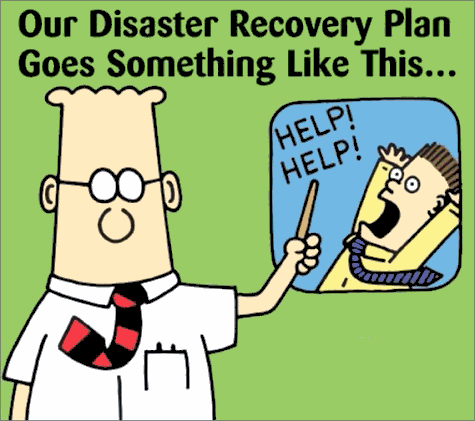
\includegraphics[height=2.1in]{our_disaster_recovery_plan.png}
  \end{center}
\end{frame}

\begin{frame}
  \frametitle{Actually, automated recovery testing}

  \begin{center}
    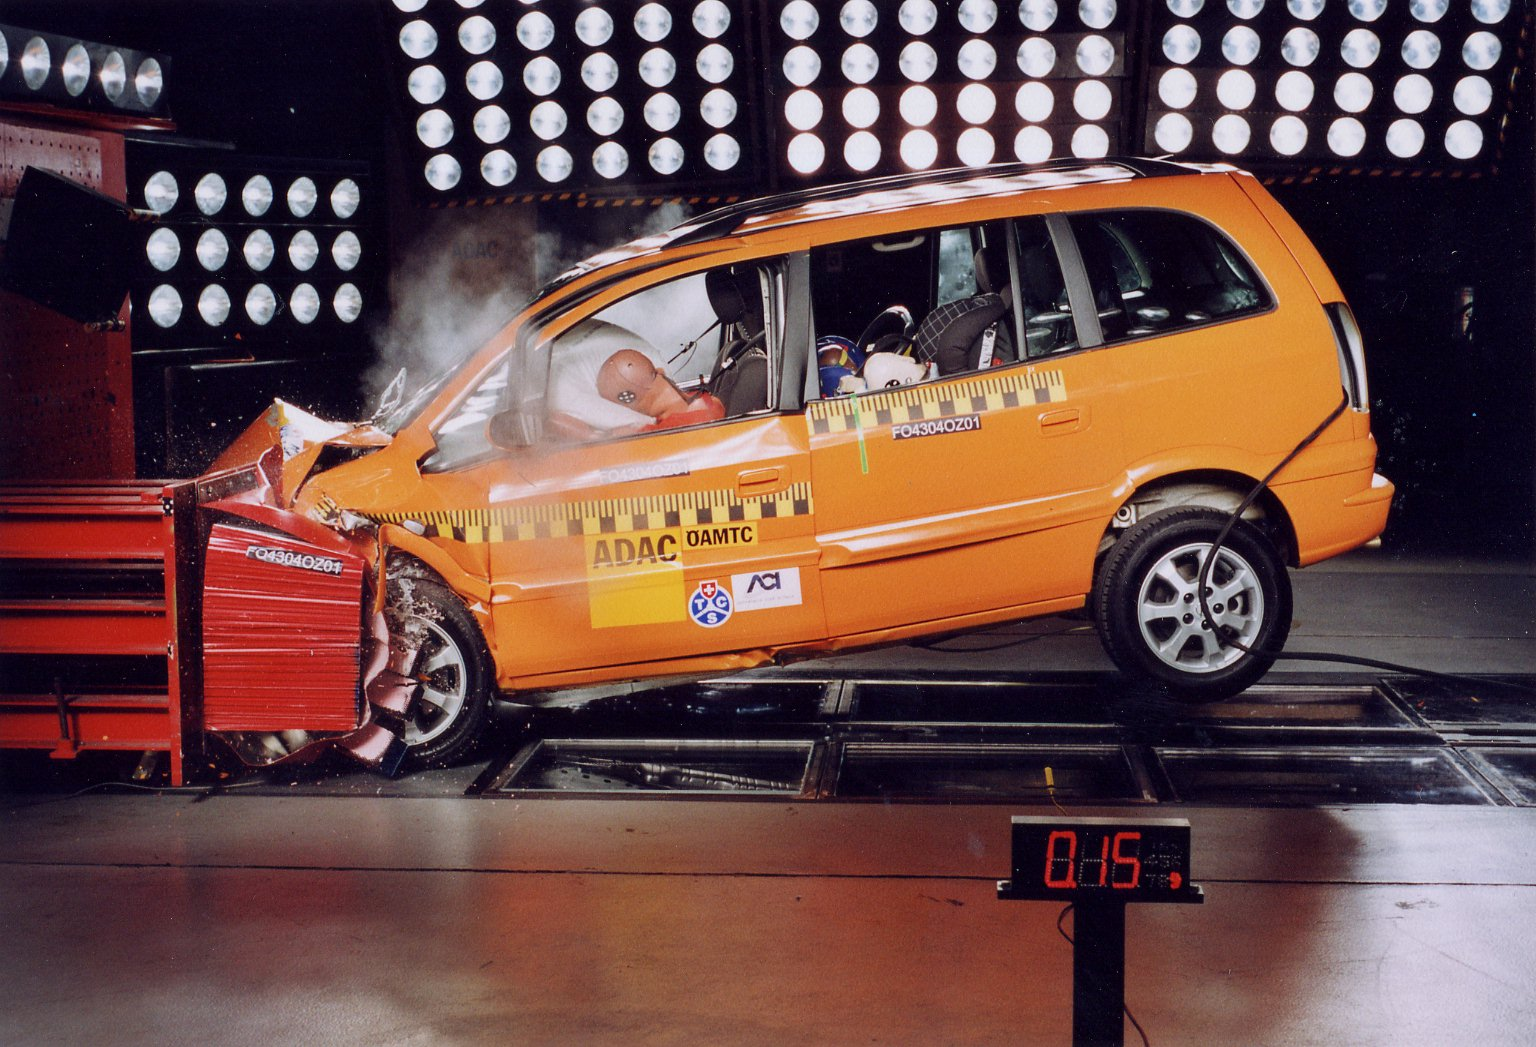
\includegraphics[height=2.1in]{crash-test.jpg}
  \end{center}
\end{frame}

\begin{frame}
  \frametitle{Use a battle tested tool}

  \center{WHY USE BARMAN? Barman: disaster recovery for business critical
    PostgreSQL databases}
  
  \begin{center}
    
\includegraphics[height=1.4in]{pgbarman.png}
  \end{center}
\end{frame}

\begin{frame}
  \frametitle{Today we're talking about what happens when you don't}

  \begin{center}
    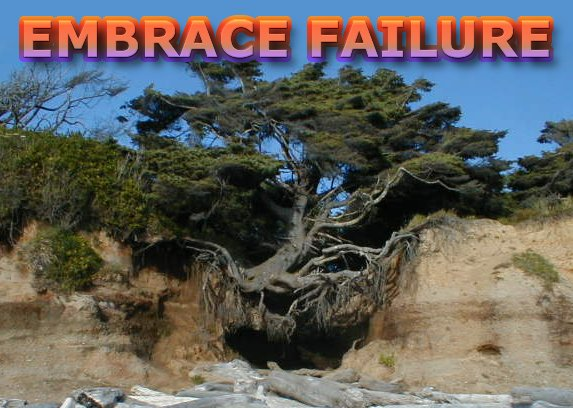
\includegraphics[height=2.4in]{resilience_logo.jpg}
  \end{center}
\end{frame}

\begin{frame}
  \frametitle{Backups? we have a shell script!}

  \begin{center}
    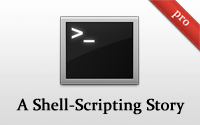
\includegraphics[height=1.6in]{a-shell-scripting-story.png}
  \end{center}
\end{frame}

\begin{frame}[fragile]
  \frametitle{Shell Script, ENV, missing setup}

  \center{\texttt{find \$PGDATA -mtime +5 | xargs rm -f}}

  \begin{center}
    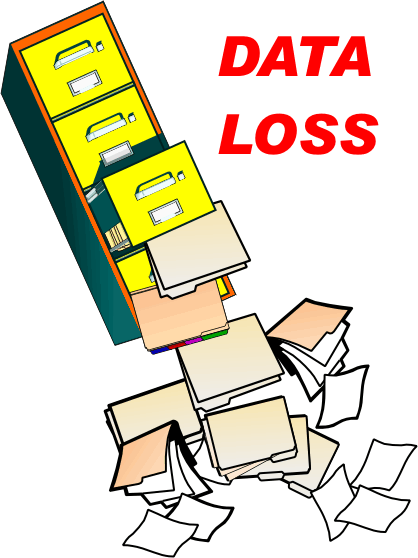
\includegraphics[height=2.4in]{data_loss.png}
  \end{center}
\end{frame}

\begin{frame}
  \frametitle{And now what?}

  \begin{center}
    
\includegraphics[height=2.4in]{Dont-Try-This-At-Home.jpg}
  \end{center}
\end{frame}

\begin{frame}[fragile]
  \frametitle{Data recovery}

  \center{Try to recover from what backups we do have: \linebreak
    only WAL files, no basebackup}

  \vfill  
  \begin{itemize}
  \item \texttt{pg\_controldata} and \texttt{xlogdump}
  \item \texttt{initdb} then
  \item \texttt{hexedit pg\_control}
  \item \texttt{5923145491842547187} to \texttt{52 33 3D 71 52 3B 3D F3}
  \item then actually \texttt{F3 3D 3B 52 71 3D 33 52}
  \item play with the WAL we have and \texttt{pg\_resetxlog}
  \item no luck this time, no working around missing WAL files
  \end{itemize}
\end{frame}

\begin{frame}
  \frametitle{Back to having that \textsc{PostgreSQL} running}

  \center{\Huge First, \textbf{backup} the physical files left available}
  \vfill
\end{frame}

\begin{frame}[fragile]
  \frametitle{Back to having that \textsc{PostgreSQL} running}
  
  \center{logs complain about \texttt{pg\_filenode.map}}
  \vfill

  \begin{columns}[c]
    \column{.15\textwidth}
    \\
    \column{.85\textwidth}
\begin{minted}{bash}
od -j 8 -N $((512-8-8)) -td4
   < $PGDATA/global/pg_filenode.map
\end{minted}
  \end{columns}
\end{frame}

\begin{frame}[fragile]
  \frametitle{Back to having that \textsc{PostgreSQL} running}

  \center{logs complain about \texttt{pg\_clog}}
  \vfill

\begin{minted}{cl}
> (code-char #b01010101)
#\U
\end{minted}

\vfill
\begin{minted}{bash}
for c in 0000 0001 0002 0003 0004 0005 \
         0006 0007 0008 0009 000A 000B 000C
do
    dd if=/dev/zero bs=256k count=1 | tr '\0' 'U' > $c
done
\end{minted}
\end{frame}

\begin{frame}
  \frametitle{Now \textsc{PostgreSQL} starts.}

  \center{But is complaining about missing \texttt{pg\_database} mappings}
  \vfill
  
  \begin{center}
    
\includegraphics[height=2.4in]{LRN-LNP-database.png}
  \end{center}
\end{frame}

\begin{frame}
  \frametitle{Now \textsc{PostgreSQL} starts.}

  \center{But is complaining about missing \texttt{pg\_database} mappings}
  \vfill
  
  \begin{center}
    
\includegraphics[height=2.4in]{LRN-LNP-database.png}
  \end{center}
\end{frame}

\begin{frame}[fragile]
  \frametitle{How to provide for your own mapping?}

  \begin{minted}{postgresql}
select oid, relname, pg_relation_filenode(oid)
  from pg_class
 where relname = 'pg_database';
 oid  |   relname   | pg_relation_filenode 
------+-------------+----------------------
 1262 | pg_database |                12319
(1 row)
  \end{minted}  
\end{frame}

\begin{frame}[fragile]
  \frametitle{How to provide for your own mapping?}

  \begin{minted}{console}
$ strings $PGDATA/global/12319
postgres
template0
template1
  \end{minted}  
\end{frame}

\begin{frame}
  \frametitle{How to provide for your own mapping?}
  
  \center{\texttt{CREATE DATABASE ... WITH OIDS ...;}}
  \vfill
  
  \begin{center}
    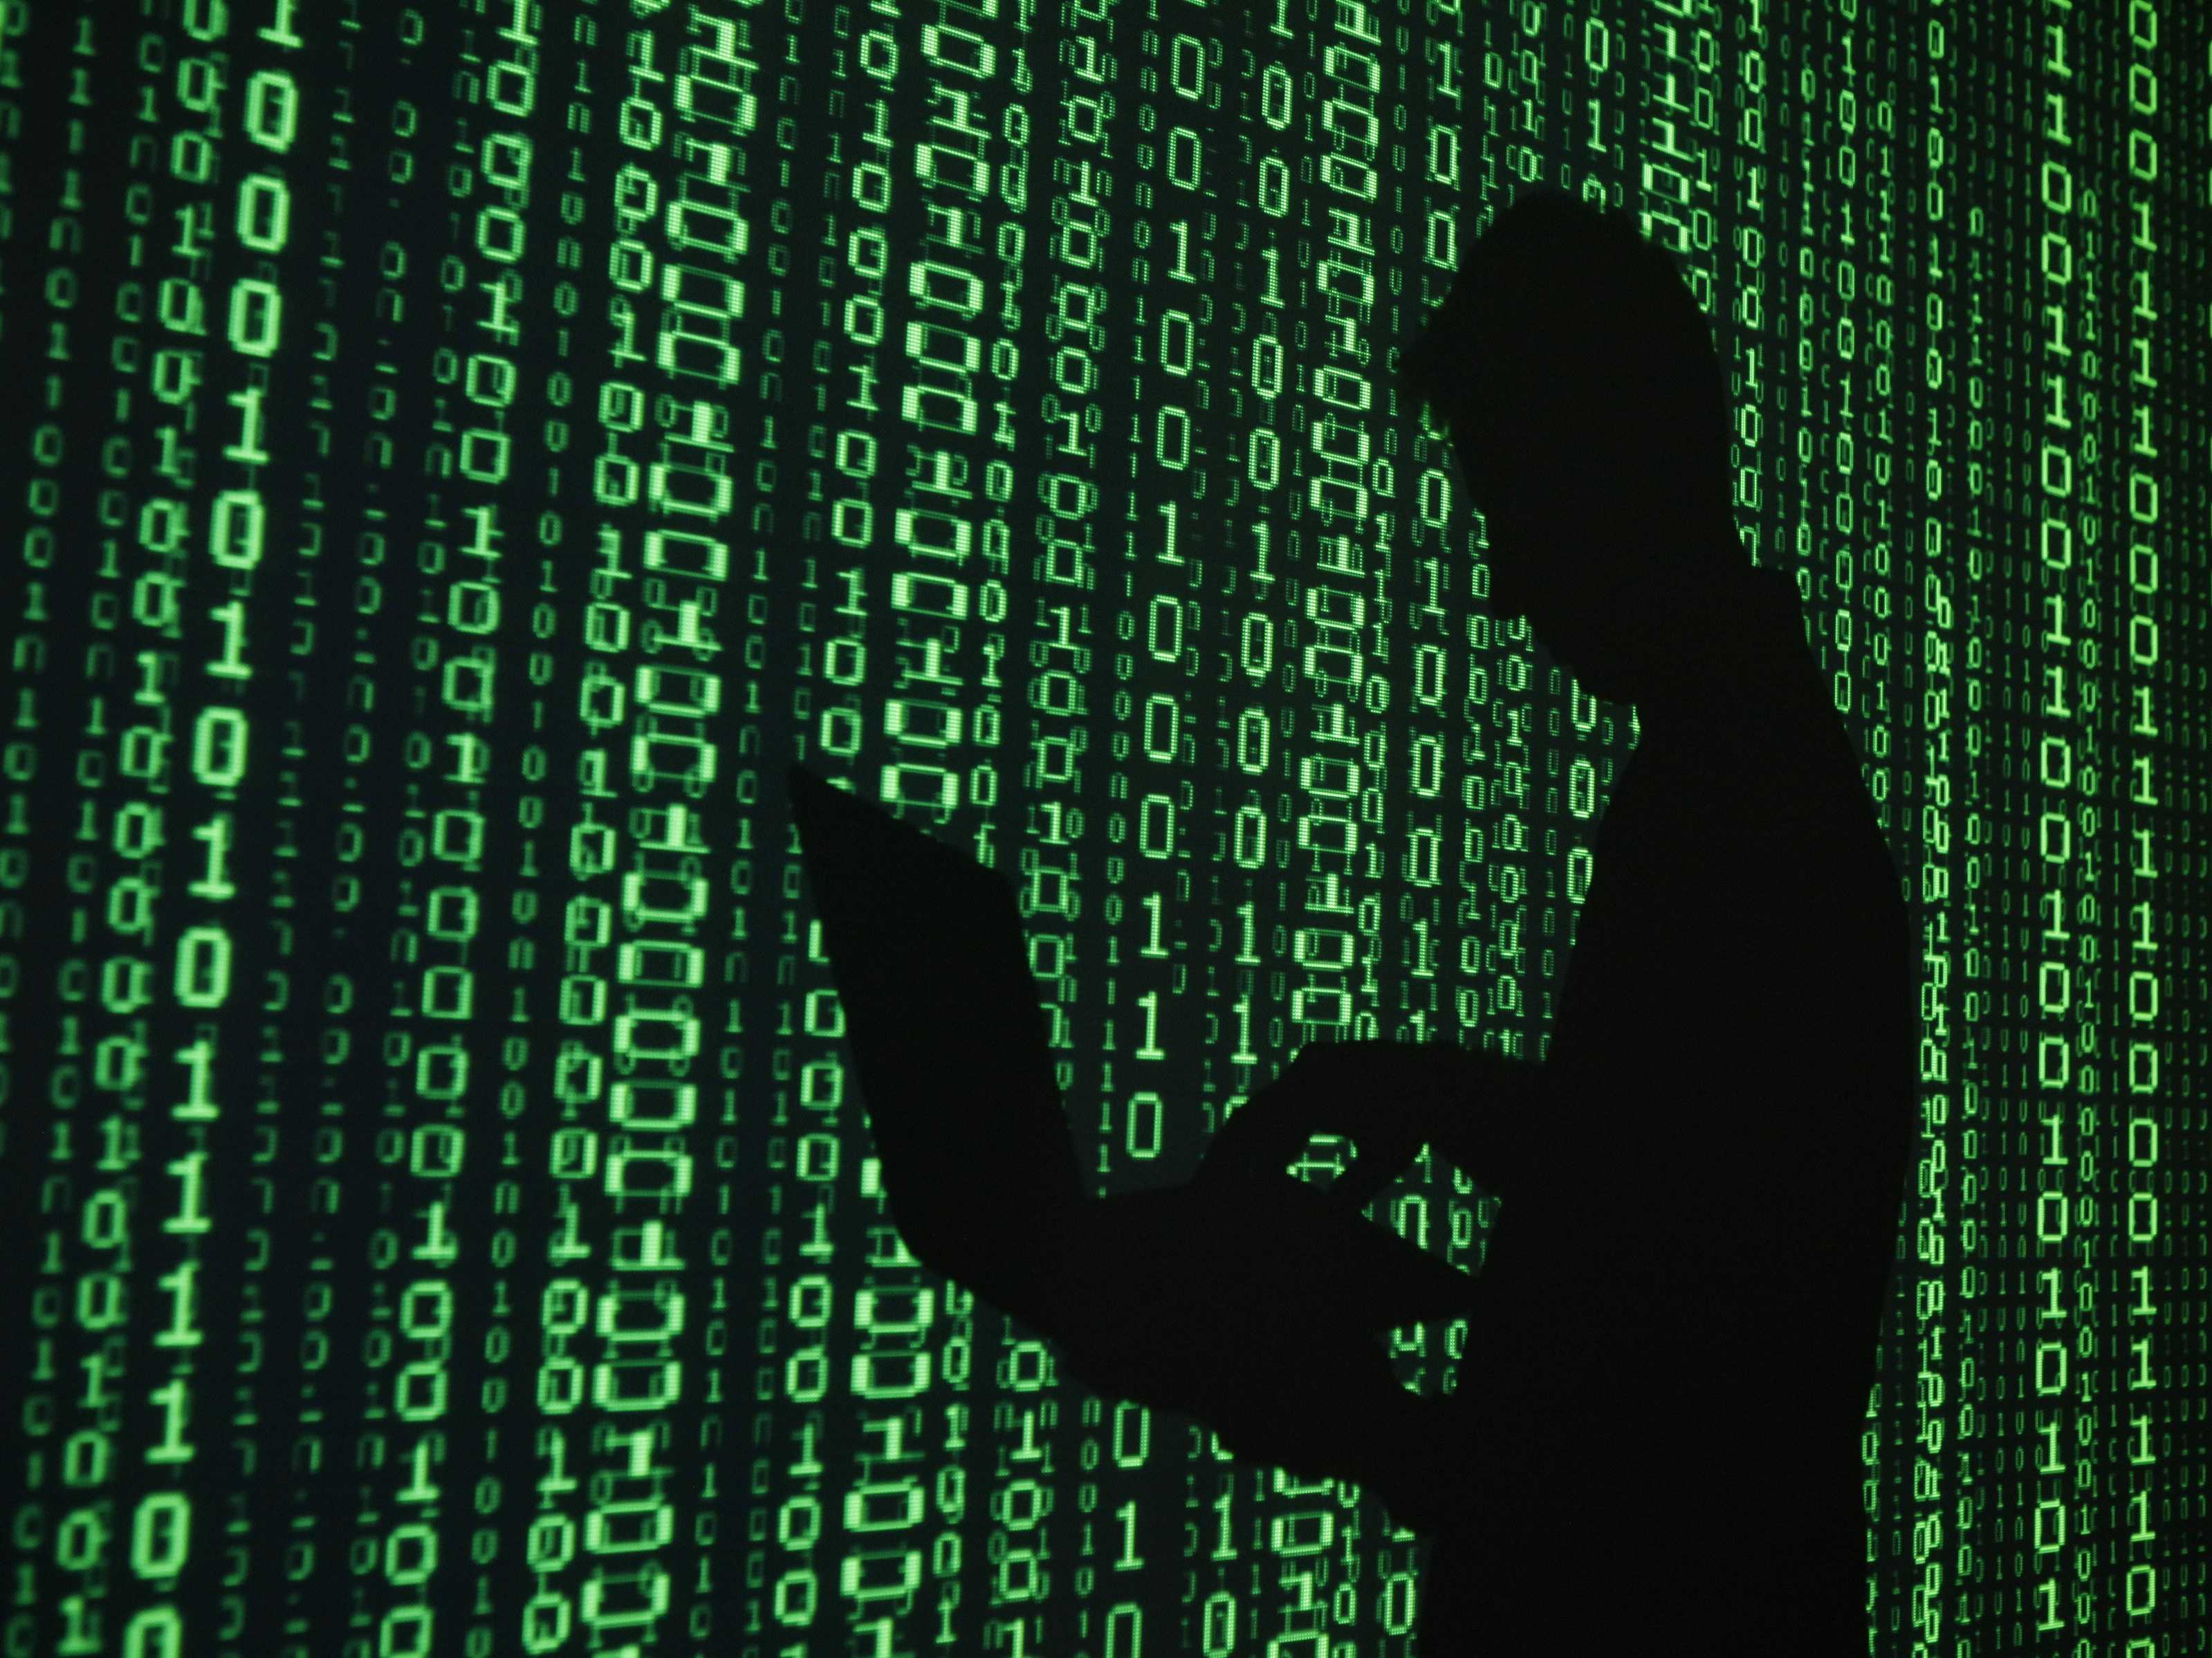
\includegraphics[height=2.4in]{Hacker-2.jpg}
  \end{center}
\end{frame}

\begin{frame}[fragile]
  \frametitle{Now we can connect to a database!}
  
  \center{Only to hit a never seen before error message:}
  \vfill

  \begin{minted}{console}
FATAL:  database "dbname" does not exists
DETAIL:  Database OID 17838 now seems to belong to "otherdb"
  \end{minted}  
\end{frame}

\begin{frame}[fragile]
  \frametitle{Start without the system indexes}
  
  \center{As one does.}
  \vfill

  \begin{minted}{console}
$ pg_ctl start -o "-P"
$ cat > $PGDATA/postgresql.conf <<EOF
	enable_indexscan = off
	enable_bitmapscan = off
	enable_indexonlyscan = off
EOF
$ pg_ctl reload
  \end{minted}  
\end{frame}

\begin{frame}[fragile]
  \frametitle{Now we can query the catalogs!}
  
  \center{\texttt{psql} and list tables, \texttt{$\backslash$dt} \newline
    but\\
    \texttt{base/16384/12062} is missing}
  \vfill

  \begin{minted}{postgresql}
  select oid, relname, pg_relation_filenode(oid)
  from pg_class
 where pg_relation_filenode(oid) = 12062;
 oid  | relname | pg_relation_filenode 
------+---------+----------------------
 1255 | pg_proc |                12062
(1 row)
  \end{minted}
\end{frame}

\begin{frame}[fragile]
  \frametitle{We lost the system catalogs...}

  \center{Copy them over from a fresh \texttt{initdb} system.}
  \vfill
  \center{Unless you did use some extensions...}  
\end{frame}


\begin{frame}[fragile]
  \frametitle{Missing \texttt{pg\_namespace}}

  \center{But the application is using \textit{custom} schemas.}
  \vfill
  
  \begin{center}
    
\includegraphics[height=2.4in]{namespace1.png}
  \end{center}
\end{frame}

\begin{frame}[fragile]
  \frametitle{How is \texttt{pg\_namespace} stored?}
  
  \begin{minted}{postgresql}
select oid, * from pg_namespace;
  oid  |      nspname       | nspowner |        nspacl        
-------+--------------------+----------+----------------------
    99 | pg_toast           |       10 | 
 11222 | pg_temp_1          |       10 | 
 11223 | pg_toast_temp_1    |       10 | 
    11 | pg_catalog         |       10 | {dim=UC/dim,=U/dim}
  2200 | public             |       10 | {dim=UC/dim,=UC/dim}
 11755 | information_schema |       10 | {dim=UC/dim,=U/dim}
(6 rows)
  \end{minted}
\end{frame}

\begin{frame}[fragile=singleslide]
  \frametitle{Figuring out the file content}
  
  \begin{minted}[tabsize=8,obeytabs,showtabs]{postgresql}
# copy pg_namespace to stdout with oids;
99	pg_toast	10	\N
11222	pg_temp_1	10	\N
11223	pg_toast_temp_1	10	\N
11	pg_catalog	10	{dim=UC/dim,=U/dim}
2200	public	10	{dim=UC/dim,=UC/dim}
11755	information_schema	10	{dim=UC/dim,=U/dim}
  \end{minted}
\end{frame}

\begin{frame}[fragile=singleslide]
  \frametitle{Add our namespaces live, with the right \texttt{OID}s}
  
  \begin{minted}[tabsize=8,obeytabs,showtabs]{postgresql}
# copy pg_namespace from stdin with oids;
Enter data to be copied followed by a newline.
End with a backslash and a period on a line by itself.
>> 16443	my_namespace	10	\N
>> \.
  \end{minted}
\end{frame}

\begin{frame}[fragile]
  \frametitle{Wait, where the \texttt{OID} is coming from?}
  
  \begin{minted}{postgresql}
# select c.oid, relname, relnamespace, nspname
    from           pg_class c
         left join pg_namespace n
                on n.oid = c.relnamespace
   where relname = 'bar';

  oid  | relname | relnamespace | nspname 
-------+---------+--------------+---------
 16446 | bar     |        16443 | 
(1 row)
  \end{minted}
\end{frame}

\begin{frame}[fragile]
  \frametitle{Now we can query the catalogs}

  \center{But what we want is the data, not the metadata.}
  \vfill
  
  \begin{center}
    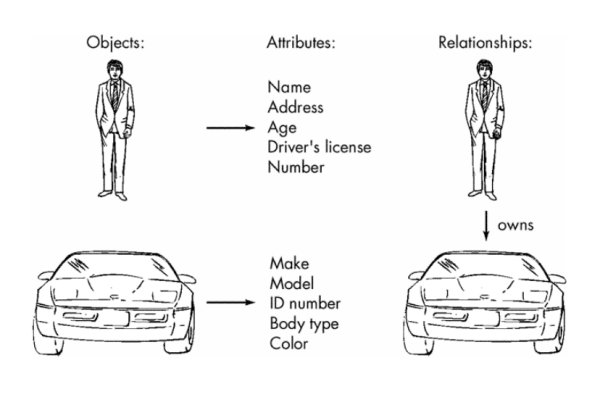
\includegraphics[height=2.4in]{relation-attributes.jpg}
  \end{center}
\end{frame}

\begin{frame}[fragile]
  \frametitle{We are lucky here!}

  \center{We didn't lose \texttt{pg\_attribute}, only \texttt{pg\_attrdef}}
  \vfill

  \begin{minted}{postgresql}
# \d a
                         Table "public.a"
 Column |  Type   |                   Modifiers                    
--------+---------+------------------------------------------------
 id     | integer | not null default nextval('a_id_seq'::regclass)
 f1     | text    | 
Indexes:
    "a_pkey" PRIMARY KEY, btree (id)
  \end{minted}
\end{frame}

\begin{frame}[fragile]
  \frametitle{What's \texttt{pg\_attrdef} like already?}

  \begin{minted}{postgresql}
#  select adrelid, adnum, adsrc
     from pg_attrdef
    where adrelid = 'public.a'::regclass;
 adrelid | adnum |             adsrc             
---------+-------+-------------------------------
   16411 |     1 | nextval('a_id_seq'::regclass)
(1 row)
  \end{minted}
\end{frame}

\begin{frame}[fragile]
  \frametitle{What's \texttt{pg\_attrdef} like already?}

  \begin{minted}{postgresql}
# select attnum, atthasdef
    from pg_attribute
   where     attrelid = 'public.a'::regclass
         and atthasdef;
 attnum | atthasdef 
--------+-----------
      1 | t
(1 row)
  \end{minted}
\end{frame}

\begin{frame}[fragile]
  \frametitle{We are not creating new data in that instance, right?}

  \begin{minted}{postgresql}
# update pg_attribute
     set atthasdef = false
   where attrelid = 'my_namespace.bar';
  \end{minted}
\end{frame}

\begin{frame}
  \frametitle{\textsc{PostgreSQL} is amazingly resilient}

  \begin{center}
    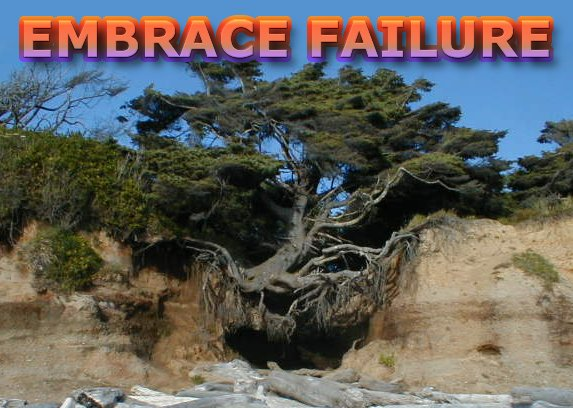
\includegraphics[height=2.4in]{resilience_logo.jpg}
  \end{center}
\end{frame}

\begin{frame}
  \frametitle{You should have a proper \textit{recovery plan}.}

  \center{WHY USE BARMAN? Barman: disaster recovery for business critical
    PostgreSQL databases}
  
  \begin{center}
    
\includegraphics[height=1.4in]{pgbarman.png}
  \end{center}
\end{frame}

\begin{frame}
  \frametitle{Questions?}

\begin{center}
  Now is the time to ask!
  \vfill

  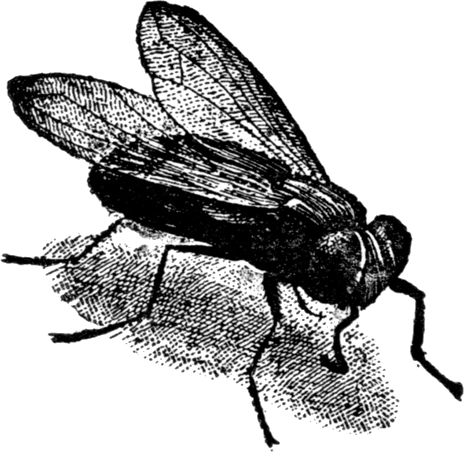
\includegraphics[height=9em]{fly.png}
\end{center}
\end{frame}

\end{document}
